



%%%%%%%%%%%%%%%%%%%%%%%%%%%%%%%%%%%%%%%%%%%%%%%%%%%%%%%%%%%%%%%%%%%%%%%%%
%%%%%%%%%%%%%%%%%%%%%%%%%%%%%%%%%%%%%%%%%%%%%%%%%%%%%%%%%%%%%%%%%%%%%%%%%
%%%%%%%%%%%%%%%%%%%%%%%%%%%%%%%%%%%%%%%%%%%%%%%%%%%%%%%%%%%%%%%%%%%%%%%%%

\begin{frame}{What makes an estimator non-robust?}

For $N=\SimNumObs$ data points, compute the OLS estimator from:

\vspace{1em}
\begin{tabularx}{\textwidth}{YYY}
%\begin{tabular}{ccc}
    Regressors  &   Residuals   &   Responses \\
    $x_n \sim \mathcal{N}(0, \sigma_x^2)$   &
    $\varepsilon_n \sim \mathcal{N}(0, \sigma_\varepsilon^2)$   &
    $y_n = \theta_0 x_n + \varepsilon_n$
\end{tabularx}
%

\SimGridNormalGraph{}

\end{frame}



%%%%%%%%%%%%%%%%%%%%%%%%%%%%%%%%%%%%%%%%%%%%%%%%%%%%%%%%%%%%%%%%%%%%%%%%%
%%%%%%%%%%%%%%%%%%%%%%%%%%%%%%%%%%%%%%%%%%%%%%%%%%%%%%%%%%%%%%%%%%%%%%%%%
%%%%%%%%%%%%%%%%%%%%%%%%%%%%%%%%%%%%%%%%%%%%%%%%%%%%%%%%%%%%%%%%%%%%%%%%%

\begin{frame}{What makes an estimator non-robust?  A tail sum.}

Report non-robustness if:
%
\begin{align*}
%
\Delta \le \thetafunlin(\w^*) - \thetafun(\thetahat)  =
    - \sum_{n=1}^{\lfloor \alpha N \rfloor} \infl_{(n)}
    =: \noise \shape
%
\end{align*}
%
We will show that:
%
\begin{itemize}
\item The ``noise'' $\noise^2 \rightarrow \mathrm{Var}(\sqrt{N}\phi)$
    \citep{hampel1986robustbook}
\item The ``shape'' $\shape \le \sqrt{\alpha (1 - \alpha)}$
    and converges to a nonzero constant
\end{itemize}

\begin{center}
\begin{minipage}{0.65\linewidth}
\begin{tikzpicture}
    \onslide<1->{
    \node[anchor=south west,inner sep=0] (image) at (0,0) {
        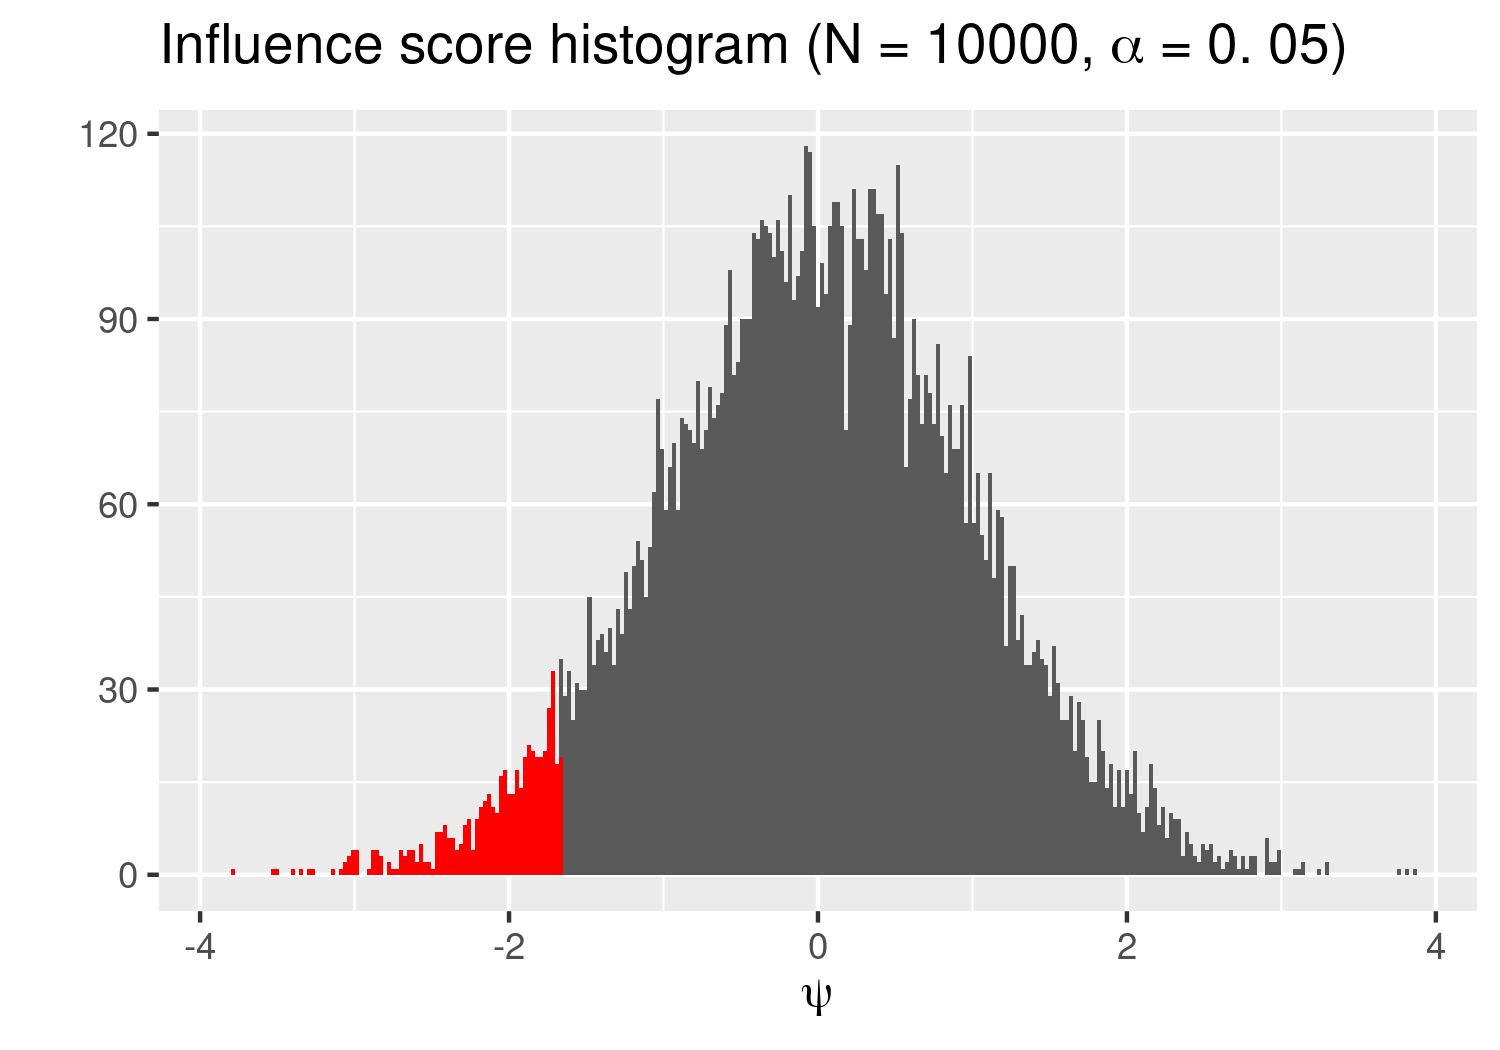
\includegraphics[width=0.98\textwidth]{static_figures/simple_infl_example.png}
    };
    }
    \onslide<1->{
    \begin{scope}[x={(image.south east)},y={(image.north west)}]
        \draw [stealth-stealth][thick][yellow](0.44, 0.4) -- (0.64, 0.4);
    \end{scope}
    \begin{scope}[x={(image.south east)},y={(image.north west)}]
        \draw (0.55,0.38) node[below,yellow][text width=3cm][align=center]
        % {\tiny $\noise$ is controlled by $\var{}{\sqrt{N}\phi(\thetahat)}$};
        {\small $\noise \approx $\\$\var{}{\sqrt{N}\phi(\thetahat)}$};
    \end{scope}
    }
    \onslide<1->{
    \begin{scope}[x={(image.south east)},y={(image.north west)}]
        \draw [stealth-][thick][red](0.3, 0.25) -- (0.3, 0.5);
    \end{scope}
    \begin{scope}[x={(image.south east)},y={(image.north west)}]
        \draw (0.25, 0.5) node[above][text width=3cm][align=center]
        {\small $-\sum_{n=1}^{\lfloor \alpha N \rfloor} \infl_{(n)}$};
    \end{scope}
    }
\end{tikzpicture}
\end{minipage}
\end{center}

\end{frame}



%%%%%%%%%%%%%%%%%%%%%%%%%%%%%%%%%%%%%%%%%%%%%%%%%%%%%%%%%%%%%%%%%%%%%%%%%
%%%%%%%%%%%%%%%%%%%%%%%%%%%%%%%%%%%%%%%%%%%%%%%%%%%%%%%%%%%%%%%%%%%%%%%%%
%%%%%%%%%%%%%%%%%%%%%%%%%%%%%%%%%%%%%%%%%%%%%%%%%%%%%%%%%%%%%%%%%%%%%%%%%

\begin{frame}[t]{Three steps:}
%
\begin{enumerate}
    \item $\inflbar_n := N \infl_n$ has a non-degenerate distribution.
    \item $\noise := \meann \inflbar_n^2$ estimates
        $\var{}{\sqrt{N}\thetafun(\thetahat)}$.
    \item $\shape :=
        \frac{-\frac{1}{N}\sum_{n=1}^{\lfloor \alpha N \rfloor}
            \inflbar_{(n)}
        }
        {\noise}
        \le \sqrt{\alpha(1-\alpha)}$ and
        converges to a constant $\ne 0$.
\end{enumerate}

\end{frame}



%%%%%%%%%%%%%%%%%%%%%%%%%%%%%%%%%%%%%%%%%%%%%%%%%%%%%%%%%%%%%%%%%%%%%%%%%
%%%%%%%%%%%%%%%%%%%%%%%%%%%%%%%%%%%%%%%%%%%%%%%%%%%%%%%%%%%%%%%%%%%%%%%%%
%%%%%%%%%%%%%%%%%%%%%%%%%%%%%%%%%%%%%%%%%%%%%%%%%%%%%%%%%%%%%%%%%%%%%%%%%

\begin{frame}[t]{Three steps:}
%
\begin{enumerate}
    \item $\inflbar_n := N \infl_n$ has a non-degenerate distribution.
\end{enumerate}

Assume that $\thetahat \plim \thetalim$ and laws of large numbers apply.

By direct computation,
%
\begin{align*}
%
\inflbar_n = N \infl_n =
\underbrace{
\fracat{\dee \thetafun(\theta)}
    {\dee \theta^T}{\thetahat}
}_{
\plim
\fracat{\dee \thetafun(\theta)}
    {\dee \theta^T}{\thetalim}
}
\underbrace{
\left(
  \frac{1}{N}
  \sum_{n'=1}^N
    \frac{\partial}{\partial \theta^T} G(\vec\theta, \d_{n'})
        \Big\vert_{\thetahat}
\right)^{-1}
}_{
\plim \expect{\d}{
    \frac{\partial}{\partial \theta^T} G(\vec\theta, \d)
    \Big\vert_{\thetalim}
    }
}
\underbrace{
G(\thetahat, \d_{n})
}_{
\plim G(\thetalim, \d_{n})
}.
%
\end{align*}
%
It follows that $\inflbar_n$ have a non-degenerate distribution
for all $N$.

\end{frame}



%%%%%%%%%%%%%%%%%%%%%%%%%%%%%%%%%%%%%%%%%%%%%%%%%%%%%%%%%%%%%%%%%%%%%%%%%
%%%%%%%%%%%%%%%%%%%%%%%%%%%%%%%%%%%%%%%%%%%%%%%%%%%%%%%%%%%%%%%%%%%%%%%%%
%%%%%%%%%%%%%%%%%%%%%%%%%%%%%%%%%%%%%%%%%%%%%%%%%%%%%%%%%%%%%%%%%%%%%%%%%


\begin{frame}[t]{Three steps:}

\begin{enumerate}
    \item $\inflbar_n := N \infl_n$ has a non-degenerate distribution.
    \item $\noise := \meann \inflbar_n^2$ estimates
        $\var{}{\sqrt{N}\thetafun(\thetahat)}$.
\end{enumerate}

% Note that $\noise$ is the sample standard deviation of $\inflbar_n$, so we
% expect $\noise$ to converge to a nonzero constant.

\textbf{Argument 1:} A linear approximation to the bootstrap.

Let $\mathrm{Boot}(\w)$ denote the distribution of random bootstrap weights.
%
\begin{align*}
%
\var{\mathrm{Boot}(\w)}{\sqrt{N} \thetafun(\thetahat)}
\approx{}&
\var{\mathrm{Boot}(\w)}{\sqrt{N} \thetafunlin(\thetahat)}
\\={}&
\var{\mathrm{Boot}(\w)}{\sqrt{N} \sumn \infl_n (\w_n - 1)}
\\={}&
\sumn N \infl_n^2
={}
\meann \inflbar_n^2
={} \noise^2.
%
\end{align*}
%

\textbf{Argument 2:} Formally, $\noise^2$ is the ``sandwich covariance''
estimator \citep{huber1967sandwich, stefanski:2002:mestimation}.

\textbf{Argument 3:} Influence functions and von Mises calculus
\citep{mises1947asymptotic, reeds1976thesis}.

\end{frame}

%%%%%%%%%%%%%%%%%%%%%%%%%%%%%%%%%%%%%%%%%%%%%%%%%%%%%%%%%%%%%%%%%%%%%%%%%
%%%%%%%%%%%%%%%%%%%%%%%%%%%%%%%%%%%%%%%%%%%%%%%%%%%%%%%%%%%%%%%%%%%%%%%%%
%%%%%%%%%%%%%%%%%%%%%%%%%%%%%%%%%%%%%%%%%%%%%%%%%%%%%%%%%%%%%%%%%%%%%%%%%


\begin{frame}[t]{Three steps:}

%
\begin{enumerate}
    \item $\inflbar_n := N \infl_n$ has a non-degenerate distribution.
    \item $\noise := \meann \inflbar_n^2$ estimates
        $\var{}{\sqrt{N}\thetafun(\thetahat)}$.
    \item $\shape :=
        \frac{-\frac{1}{N}\sum_{n=1}^{\lfloor \alpha N \rfloor}
            \inflbar_{(n)}
        }
        {\noise}
        \le \sqrt{\alpha(1-\alpha)}$ and
        converges to a constant $\ne 0$.
\end{enumerate}

By definition,
%
\begin{align*}
%
-\sum_{n=1}^{\lfloor \alpha N \rfloor} \infl_{(n)}
    =: \noise \shape
\quad\quad\Rightarrow\quad\quad
\shape
% := -\sum_{n=1}^{\lfloor \alpha N \rfloor} \frac{\infl_{(n)}}{\noise}
= -\frac{1}{N}
    \sum_{n=1}^{\lfloor \alpha N \rfloor} \frac{\inflbar_{(n)}}{\noise}.
%
\end{align*}
%
By Cauchy-Schwartz,
%
\begin{align*}
%
\shape \le
\underbrace{
\left(
\meann \frac{\inflbar_{n}^2}{\noise^2}
\right)^{1/2}
}_{=1}
\left(\meann \ind{n \le \alpha N }^2 \right)^{1/2} \le \sqrt{\alpha}
%
\end{align*}
%
A slightly more careful analysis which accounts for
the fact that $\sumn \infl_n = 0$ gives $\shape \le \sqrt{\alpha(1-\alpha)}$.

% (Using $\sumn \infl_n = 0$).

\end{frame}

%
% %%%%%%%%%%%%%%%%%%%%%%%%%%%%%%%%%%%%%%%%%%%%%%%%%%%%%%%%%%%%%%%%%%%%%%%%%
% %%%%%%%%%%%%%%%%%%%%%%%%%%%%%%%%%%%%%%%%%%%%%%%%%%%%%%%%%%%%%%%%%%%%%%%%%
% %%%%%%%%%%%%%%%%%%%%%%%%%%%%%%%%%%%%%%%%%%%%%%%%%%%%%%%%%%%%%%%%%%%%%%%%%
%
% \begin{frame}[t]{Three steps:}
% %
% \begin{enumerate}
%     \item $\inflbar_n := N \infl_n$ has a non-degenerate distribution.
%     \item $\noise := \meann \inflbar_n^2$ estimates
%         $\var{}{\sqrt{N}\thetafun(\thetahat)}$.
%     \item $\shape :=
%         \frac{-\frac{1}{N}\sum_{n=1}^{\lfloor \alpha N \rfloor}
%             \inflbar_{(n)}
%         }
%         {\noise}
%         \le \sqrt{\alpha(1-\alpha)}$ and
%         converges to a constant $\ne 0$.
% \end{enumerate}
%
%
% Report non-robustness if:
% %
% \begin{align*}
% %
% \Delta \le \thetafunlin(\w^*) - \thetafun(\thetahat)  = \noise \shape
% \quad\quad
% \Leftrightarrow
% \quad\quad
% \frac{\Delta}{\noise} \le \shape.
% %
% \end{align*}
% %
% We call $\frac{\Delta}{\noise}$ the ``signal to noise ratio.''
%
% \end{frame}





%%%%%%%%%%%%%%%%%%%%%%%%%%%%%%%%%%%%%%%%%%%%%%%%%%%%%%%%%%%%%%%%%%%%%%%%%
%%%%%%%%%%%%%%%%%%%%%%%%%%%%%%%%%%%%%%%%%%%%%%%%%%%%%%%%%%%%%%%%%%%%%%%%%
%%%%%%%%%%%%%%%%%%%%%%%%%%%%%%%%%%%%%%%%%%%%%%%%%%%%%%%%%%%%%%%%%%%%%%%%%

\begin{frame}{Corollaries.}

% {\small
% \textbf{Key quantities:}\\
% \pause $\alpha$  = The proportion of left out points\\
% \pause $\Delta$  = The signal = The change in $\phi$ that would alter your
% conclusion\\
% \pause $\noise^2$ = The noise = A consistent estimator of
% $\mathrm{Var}(\sqrt{N}\phi)$\\
% \pause $\shape$ =
%     The shape = Converges to a nonzero constant, $\le \sqrt{\alpha(1-\alpha)}$\\
% }

Report non-robustness if:
%
\begin{align*}
%
\Delta \le \thetafunlin(\w^*) - \thetafun(\thetahat)  = \noise \shape
\quad\quad
\Leftrightarrow
\quad\quad
\frac{\Delta}{\noise} \le \shape.
%
\end{align*}
%
We call $\frac{\Delta}{\noise}$ the ``signal to noise ratio.''


\hrulefill

%\vspace{-1em}

\pause
\vspace{0.5em}
\textbf{Corollary:  Non-robustness possible even with correct specification.}
%\vspace{-0.4em}
% {\small The noise $\noise$ may be larger than the effect
% $\Delta$ you're trying to measure.}

\pause
\vspace{0.5em}
\textbf{Corollary:  Leave-$\lfloor \alpha N \rfloor$-out robustness does not vanish as $N \rightarrow \infty$.}
% \vspace{-0.4em}
%
% Both $\shape$ and $\noise$ typically converge to nonzero constants.

\pause
\vspace{0.5em}
Recall that standard errors reject when
$\frac{\Delta}{\noise} \le \frac{1.96}{\sqrt{N}}$.

\pause
\vspace{0.5em}
\textbf{Corollary:  Leave-$\lfloor \alpha N \rfloor$-out is different from standard errors.}
%\vspace{-0.4em}
% $1.96 / \sqrt{N} \ne \shape$

\pause
\vspace{0.5em}
\textbf{Corollary:  Insignificance is always non-robust.}
%\vspace{-0.4em}

Take $\Delta = \frac{1.96 \hat \sigma_\phi}{\sqrt{N}} \rightarrow 0 \le
\shape$.

\pause
\vspace{0.5em}
\textbf{Corollary:  Gross outliers primarily affect robustness
through $\noise$.}
%\vspace{-0.4em}
Cauchy-Schwartz is tight when all the influence scores are the same.

\end{frame}
